%%%%%%%%%%%%%%%%%%%%%%%%%%%%%%%%%%%%%%%%%
% Short Sectioned Assignment
% LaTeX Template
% Version 1.0 (5/5/12)
%
% This template has been downloaded from:
% http://www.LaTeXTemplates.com
%
% Original author:
% Frits Wenneker (http://www.howtotex.com)
%
% License:
% CC BY-NC-SA 3.0 (http://creativecommons.org/licenses/by-nc-sa/3.0/)
%
% Download template:
% Overleaf (https://www.overleaf.com/8746855dtrgkbkbjjhm)
%
%%%%%%%%%%%%%%%%%%%%%%%%%%%%%%%%%%%%%%%%%

%----------------------------------------------------------------------------------------
%	PACKAGES AND OTHER DOCUMENT CONFIGURATIONS
%----------------------------------------------------------------------------------------

\documentclass[paper=a4, fontsize=11pt]{scrartcl} % A4 paper and 11pt font size

%\usepackage[options]{nohyperref}  % This makes hyperref commands do nothing without errors
%\usepackage{url}  % This makes \url work
%\usepackage{hyperref}

\usepackage{graphicx}

\usepackage[T1]{fontenc} % Use 8-bit encoding that has 256 glyphs
\usepackage{fourier} % Use the Adobe Utopia font for the document - comment this line to return to the LaTeX default
\usepackage[english]{babel} % English language/hyphenation
\usepackage{amsmath,amsfonts,amsthm} % Math packages

\usepackage{lipsum} % Used for inserting dummy 'Lorem ipsum' text into the template

\usepackage{sectsty} % Allows customizing section commands
\allsectionsfont{\centering \normalfont\scshape} % Make all sections centered, the default font and small caps

\usepackage{fancyhdr} % Custom headers and footers
\pagestyle{fancyplain} % Makes all pages in the document conform to the custom headers and footers
\fancyhead{} % No page header - if you want one, create it in the same way as the footers below
\fancyfoot[L]{} % Empty left footer
\fancyfoot[C]{} % Empty center footer
\fancyfoot[R]{\thepage} % Page numbering for right footer
\renewcommand{\headrulewidth}{0pt} % Remove header underlines
\renewcommand{\footrulewidth}{0pt} % Remove footer underlines
\setlength{\headheight}{13.6pt} % Customize the height of the header

\numberwithin{equation}{section} % Number equations within sections (i.e. 1.1, 1.2, 2.1, 2.2 instead of 1, 2, 3, 4)
\numberwithin{figure}{section} % Number figures within sections (i.e. 1.1, 1.2, 2.1, 2.2 instead of 1, 2, 3, 4)
\numberwithin{table}{section} % Number tables within sections (i.e. 1.1, 1.2, 2.1, 2.2 instead of 1, 2, 3, 4)

%\setlength\parindent{0pt} % Removes all indentation from paragraphs - comment this line for an assignment with lots of text
\usepackage{indentfirst} % Indentation for all paragraphs

% Used for definitions:
\usepackage{amsthm}
\theoremstyle{definition}
\newtheorem{definition}{Definition}[section]

% To write algorithms in pseudocode:
\usepackage{algpseudocode}
\usepackage{algorithm}

% To put images side by side:
\usepackage{subcaption}

% URL available:
\usepackage{url}

% Don't use colon in algorithms lines:
\algrenewcommand\alglinenumber[1]{\footnotesize #1}

% Input/Output instead of Require/Ensure in algorithms pseudocode:
\renewcommand{\algorithmicrequire}{\textbf{Input:}}
\renewcommand{\algorithmicensure}{\textbf{Output:}}

%----------------------------------------------------------------------------------------
%	TITLE SECTION
%----------------------------------------------------------------------------------------

\newcommand{\horrule}[1]{\rule{\linewidth}{#1}} % Create horizontal rule command with 1 argument of height

\title{	
\normalfont \normalsize 
\textsc{Sapienza University of Rome} \\ [25pt] % Your university, school and/or department name(s)
\horrule{0.5pt} \\[0.4cm] % Thin top horizontal rule
\huge Interactive Graphics \\ % The assignment title
\large Final Project: Procedural Solar System \\
\horrule{2pt} \\[0.5cm] % Thick bottom horizontal rule
}

\author{Michele Cipriano, Ivan Bergonzani} % Your name

\date{\normalsize\today} % Today's date or a custom date

\begin{document}

\maketitle % Print the title

%----------------------------------------------------------------------------------------

\section{Introduction}

The theme of the project is about the generation of a solar system using
procedural graphics. The aim is to study in depth procedural meshes developing
a system that ease the creation of pseudorandomly generated planets.

The program is characterized by having a solar system composed by four planets,
a star, a satellite (the Sun, the first four planets of our solar system and the
Moon, orbiting the Earth) and a cloud of asteroids. The sun also has a particle system that simulates its surface activity while the Earth has oceans and an atmosphere. Moreover each object between the planets, the sun and the moon is matched with a graphical label which contains informations about the associatedcelestial corp. The meshes are generated using Perlin noise, each
planet is composed by multiple chunks which change definition depending on
the distance, allowing high performances even with a high number of details.
The system supports multiple lights and textures, managed in shaders developed
with GLSL. Objects are animated with rotation around themselves and
revolution around the parents' object (the Sun for the planets, the Earth for
the Moon). A simple flying system has been implemented with the help of
THREE.js \cite{threejs}, which simplifies the development of the whole program as well.
Moreover it is possible to interact with the scene through an apposite menu.
Finally a collision system was implemented in order to avoid the user to move the camera inside the planets or the sun.

The program obtains optimal performances running smoothly both when the
camera is far away, where all the objects can be seen altogether, and when the camera
is near a planet, where seas, plains and mountains can be seen in detail.

%----------------------------------------------------------------------------------------

\section{Perlin Noise}

The main character of the project is the Perlin noise, resposible for the
generation of the pseudorandom meshes of the planets.

Against regular noise, where each pixel has assigned a random value between 0
and 1, changes occur gradually in Perlin noise, as in natural terrains.

To generate realistic terrains it's necessary to add multiple noise maps
together (called octaves), each of which has different amplitude and frequency,
determined by the parameters lacunarity and persistance. These two are
responsible for the number of small features of the terrain and how much
these features change the shape of it.

Noise values are used to determine the height of the terrain for each vertex of
the planet. To do this without loosing continuity between adjacent vertices, a 3D
Perlin noise function has been implemented passing as parameters the points of
a hypothetical sphere. Hence, for a point $(x, y, z)$ on the sphere there is a
corresponding height $h$.
The algorithm for the generation of the heights is
Algorithm \ref{algorithm:noise3D}. Note that the number of octaves, the persistance,
the lacunarity and the scale are constant values (choosen before the execution
of the function). The scale value directly affects the frequency of the function.
An external \textsc{Perlin} function is used to compute the gradient noise.

\begin{algorithm}
	\caption{Noise height generator.}
	\label{algorithm:noise3D}
	\begin{algorithmic}[1]
		\Function{noiseHeight}{$x$, $y$, $z$}
			\State $amplitude \gets 1$
			\State $frequency \gets 1$
			\State $h \gets 0$
			\For {$oct \gets 1$ \textbf{to} $octaves$}
				\State $sampleX \gets x$ / $scale * frequency$
				\State $sampleY \gets y$ / $scale * frequency$
				\State $sampleZ \gets z$ / $scale * frequency$
				
				\State $h \gets h$ + \textsc{Perlin}$(sampleX, sampleY, sampleZ) * amplitude$
				
				\State $amplitude \gets amplitude * persistance$
				\State $frequency \gets frequency * lacunarity$
			\EndFor
			\State \Return $h$
		\EndFunction
	\end{algorithmic}
\end{algorithm}

%----------------------------------------------------------------------------------------

\section{Planet Generation}

The first thing that comes to mind when creating a planet is to use a spherical
geometry. Nevertheless the sphere has several drawbacks when dealing with
chunks, when changing the level of detail (to preserve performances) and, in
particular, when textures are handled. These are, in fact, stretched at the poles,
creating a bad graphical effect that ruins the realism of the whole planet.

A solution is to use a cube and ``spherify'' it by modifying its vertices.
In this way the triangles of the geometry will have a similar size and the
stretching of the texture will be solved.

While this method solves the problem, a cube geometry is not suitable for chunks
and level of details (LOD). In fact, it's
necessary to divide the faces of the cube in multiple parts (chunks),
and change the resolution of these depending on the distance from the camera.
This is exactly what happens in graphic engines when huge terrains are
rendered.

A solution is to compose the cube using multiple planes, each plane will
behave like a chunk and will change its resolution dinamically using LODs.
In particular, each face of the cube is divided in $N*N$ chunks, hence, a
planet is composed by $6*N*N$ chunks.

Vertices of the chunks are initialized using Perlin noise. The height of each
vertex w.r.t. the center of the earth is determined by first spherifying the
vertex itself and then computing the noise height in that point.

%----------------------------------------------------------------------------------------

\section{Chunks}

As said before, planets are made of parts called chunks. Each chunk, in the
implementation, is actually an element of a LOD object, multiple chunks of a
LOD determine how the resolution of the terrain changes with distance.
In this case, even if it's defined with a plane geometry, the chunk it's
a custom geometry which follows the curvature of the planet.

Choosing the number of chunks which compose the planet is important both to
have high details and to have good performances. In particular, a low number
of chunks improves the performances when the camera is far away; this is due
to the fact that all the meshes of all the planets in the viewport must be
rendered. A high number of chunks increases the number of details, but
must not be too high, otherwise the performances will be bad when moving away
from the planet. The number of chunks can be decreased by increasing the
number of vertices of each chunk obtaining the same level of details.
Nevertheless, this number shouldn't be
too high otherwise the rendering will be slow when approaching the planet. 

One of the problem of creating a terrain with multiple meshes instead of just
one is the wrong value assigned to the normals at the border. This is due to
the fact that normals are computed considering the adjacent vertices, which
are not available for the vertices at the borders of the mesh.

A simple solution is to define an extended chunk which overlaps the
chunk that will be used for the planet, but contains a new, bigger border.
In this way the value of the normals of the extended chunk, with the exception
of its border, can be copied back to the original chunk, which will then have
correct normals also at the border. This eliminates the difference of colors
at borders of the chunks, making the planet look like a single piece.

%----------------------------------------------------------------------------------------

\section{LOD}

Dividing the planet in multiple pieces is not enough to obtain good
performances, this is why level of details (LOD) are used when building
terrains.

The idea is simple, instead of composing the planet with multiple chunks,
the planet is composed by multiple LOD objects that contain the same
chunk with different amounts of vertices. Thus, the same chunk is ``computed
more times'' with different details. Then, at rendering time, each LOD
object is updated depending on the position of the camera, in this way it's
possible to gradually change the amount of vertices of the mesh while
approaching the planet (Figure \ref{fig:LOD-venus}).

Choosing the right amount of LODs' chunks its important to have good
performances both while being far away from a planet and while approaching it.
In particular, this allows the GPU to handle a lower number of vertices
for the planets distant from the camera, making it possible to have more
resources for the closer meshes, that needs to be more detailed.

\begin{figure}
	\centering
	\begin{subfigure}{.3\textwidth}
		\centering
		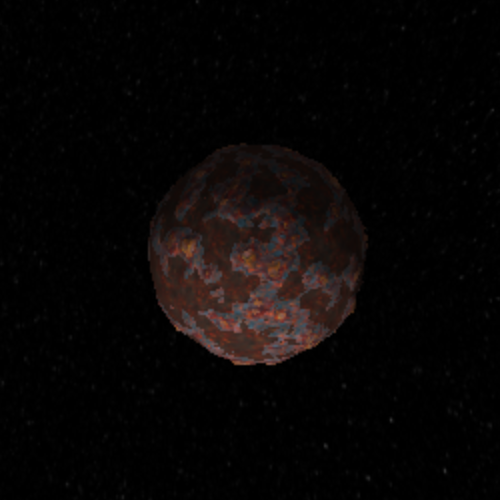
\includegraphics[width=1.0\linewidth]{images/venus_d0.png}
	\end{subfigure}
	\begin{subfigure}{.3\textwidth}
		\centering
		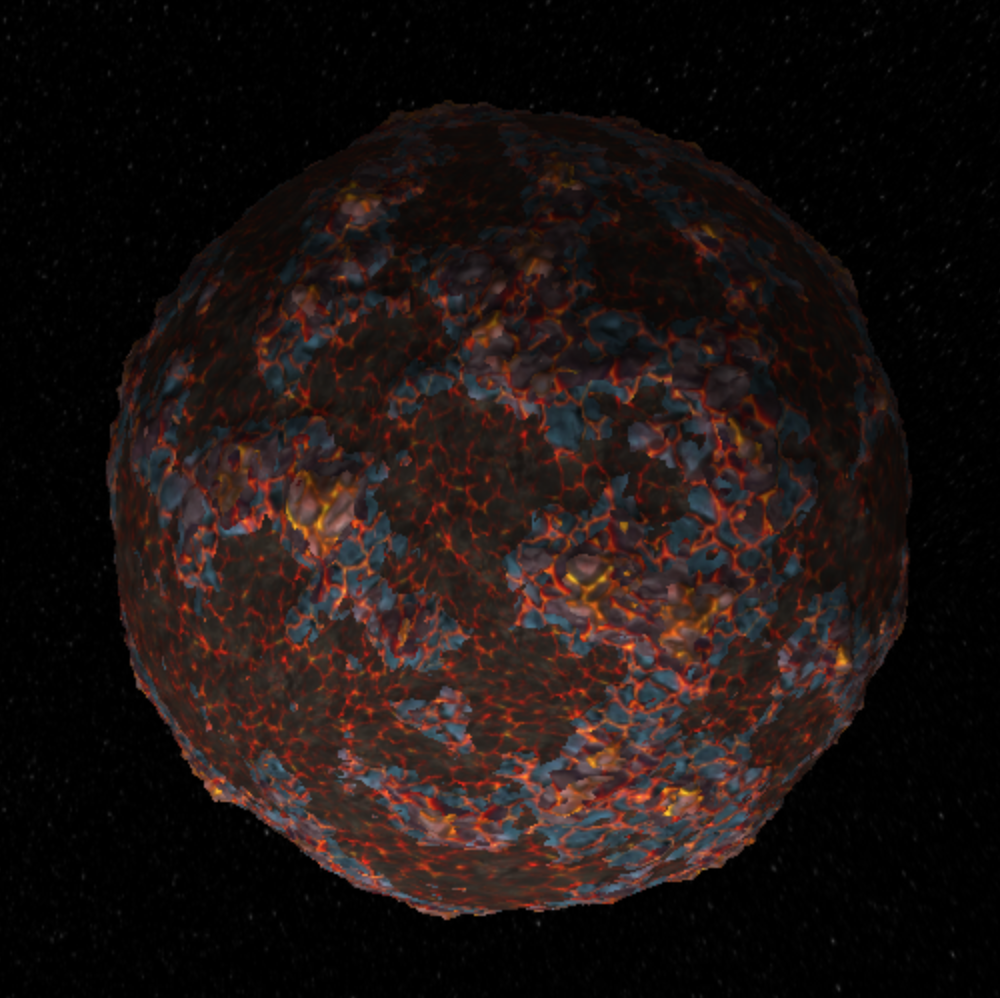
\includegraphics[width=1.0\linewidth]{images/venus_d1.png}
	\end{subfigure}
	\begin{subfigure}{.3\textwidth}
		\centering
		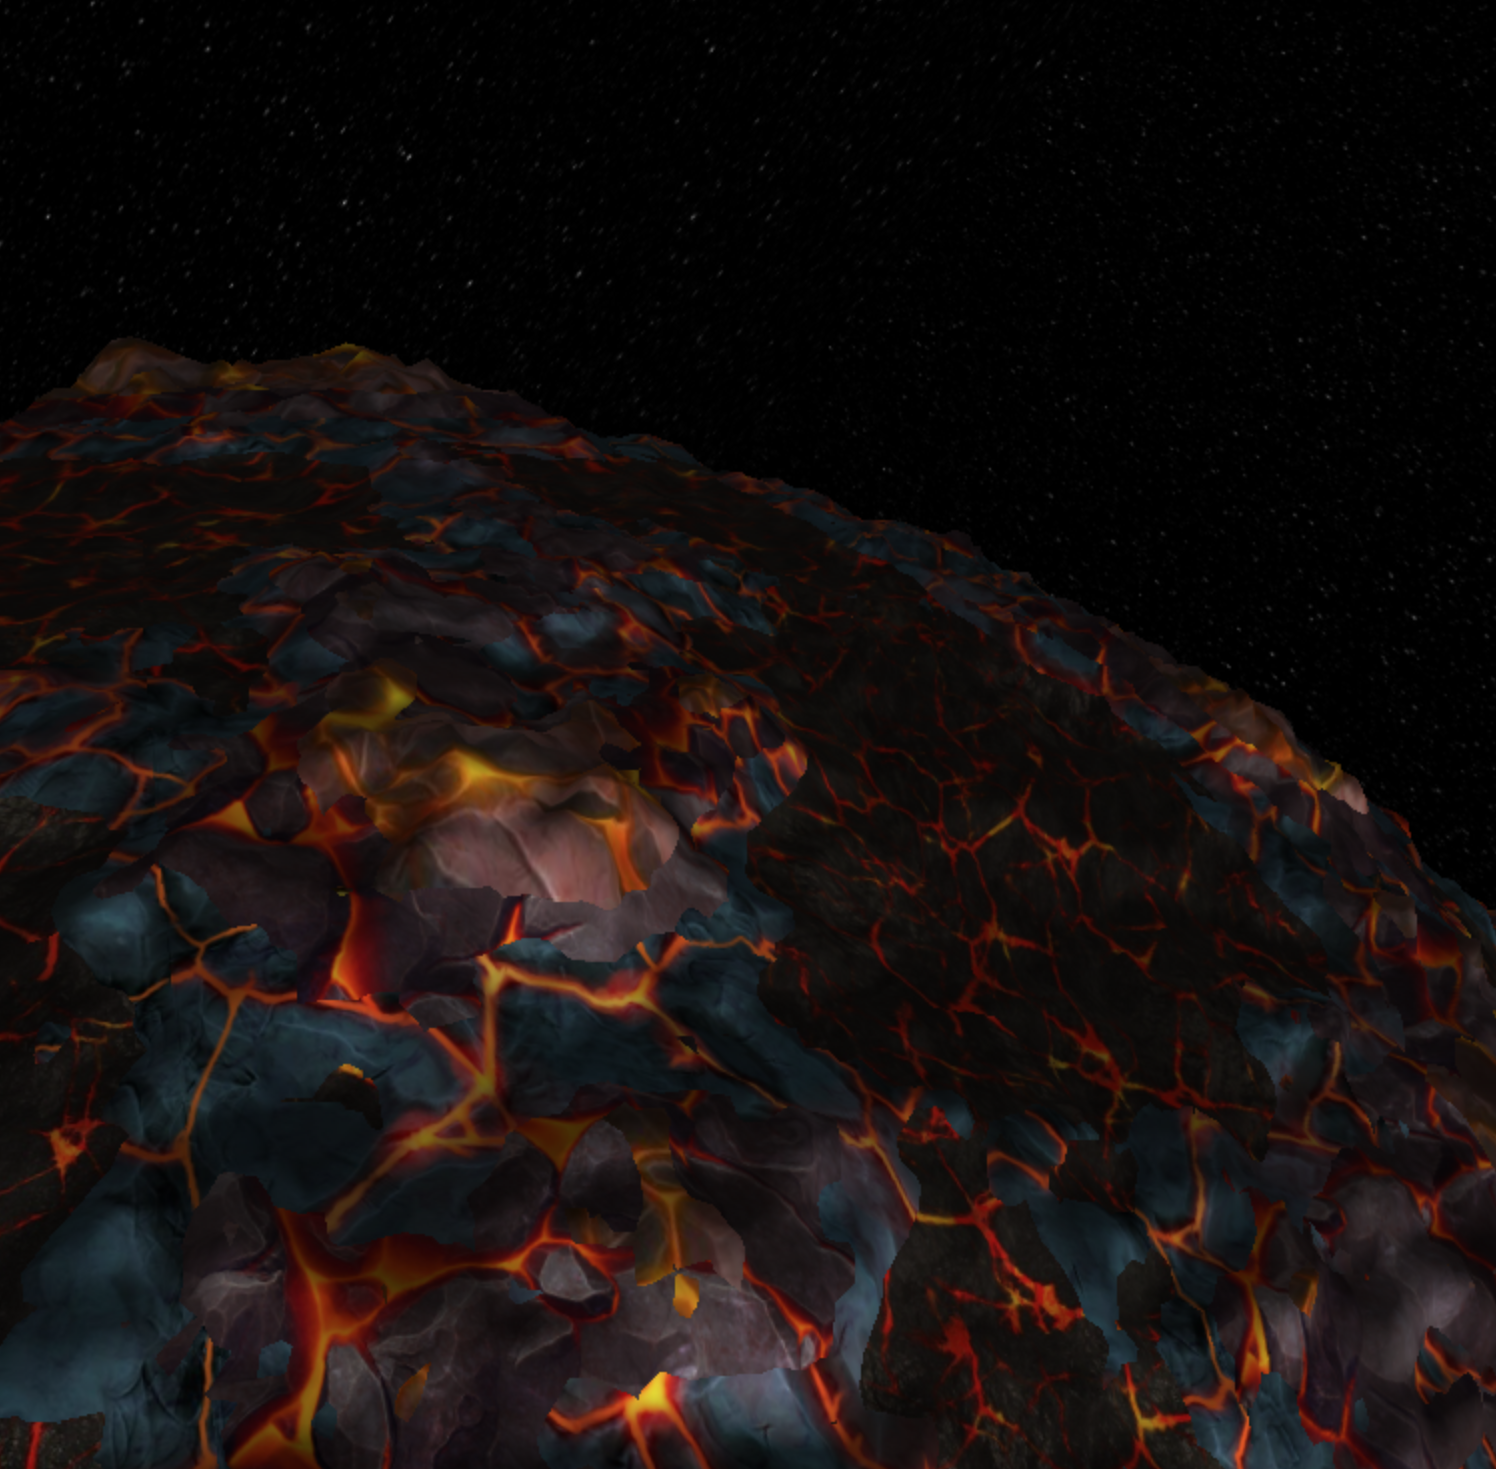
\includegraphics[width=1.0\linewidth]{images/venus_d2.png}
	\end{subfigure}
	\caption{Level of detail increases while approaching Venus.}
	\label{fig:LOD-venus}
\end{figure}

%----------------------------------------------------------------------------------------

\section{Lights}

THREE.js simplifies a lot the management of the lights even when a custom
shader is used, like in the case of this program. Here two point lights are used
in the scene, one for the Sun and one for the Moon (Figure \ref{fig:earth-moon-light}). Lights are directly added
as a child of the Planet in the hierarchical structure, making it easy to
manage their movement. Since the custom shader increases the flexibility in
the development,
the parameter ``distance'' of each light has been used to determine for how much
distance the lights affects the objects, instead of being used to compute the
attenuation value.

The shader supports also the light emitted by the planet, used to make the Sun,
the Moon and Venus brighter.

\begin{figure}
	\centering
	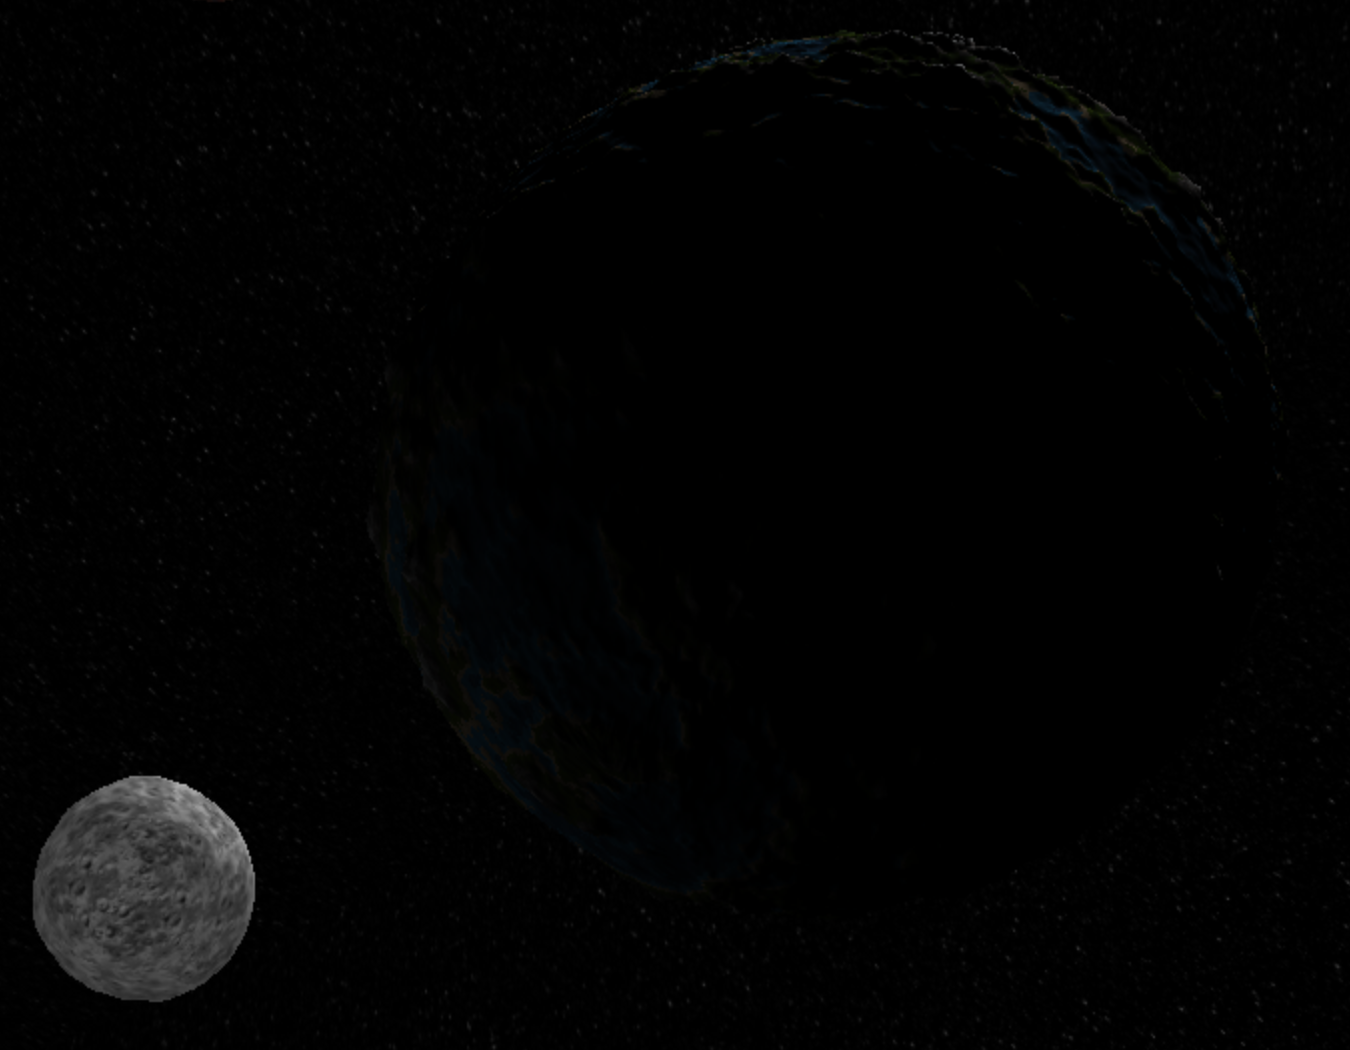
\includegraphics[scale=0.25]{images/earth_moon.png}
	\caption{The light of the Moon affects the color of the Earth.}
	\label{fig:earth-moon-light}
\end{figure}

%----------------------------------------------------------------------------------------

\section{Fly Control}

User interaction has been developed with a tool of THREE.js called FlyControl,
which has been used for the creation of a simple flying system that allows to
move around the solar system.

FlyControl manages the position and the orientation of the camera taking
movements from the keyboard and the mouse.

%----------------------------------------------------------------------------------------

\section{Animation}

The solar system is composed by the Sun, positioned at the center of the scene,
four planets orbiting around the Sun which have similar characteristics to
Mercury, Venus, the Earth and Mars, and the Moon, which is orbiting around the
Earth. Moreover all these objects are rotating around themselves (Figure
\ref{fig:solar-system}).

The implementation of the orbital revolution is quite straightforward, it's necessary
in fact, to slightly change the position of the planets following a
circular path. Since this movement must affects also the children in the scene,
nothing else has to be done.

On the other hand, the rotation has to be
managed in a different way, otherwise the children will rotate with the
rotation of the parent. To solve this problem, instead of adding the LOD objects
directly to the planet, a pivot object is used. This object is added to the
planet and it's, in turn, parent of all the LOD objects of the planet itself.
Thus, instead of
rotating the planet, only the pivot is rotated, preserving the position of
the children.

\begin{figure}
	\centering
	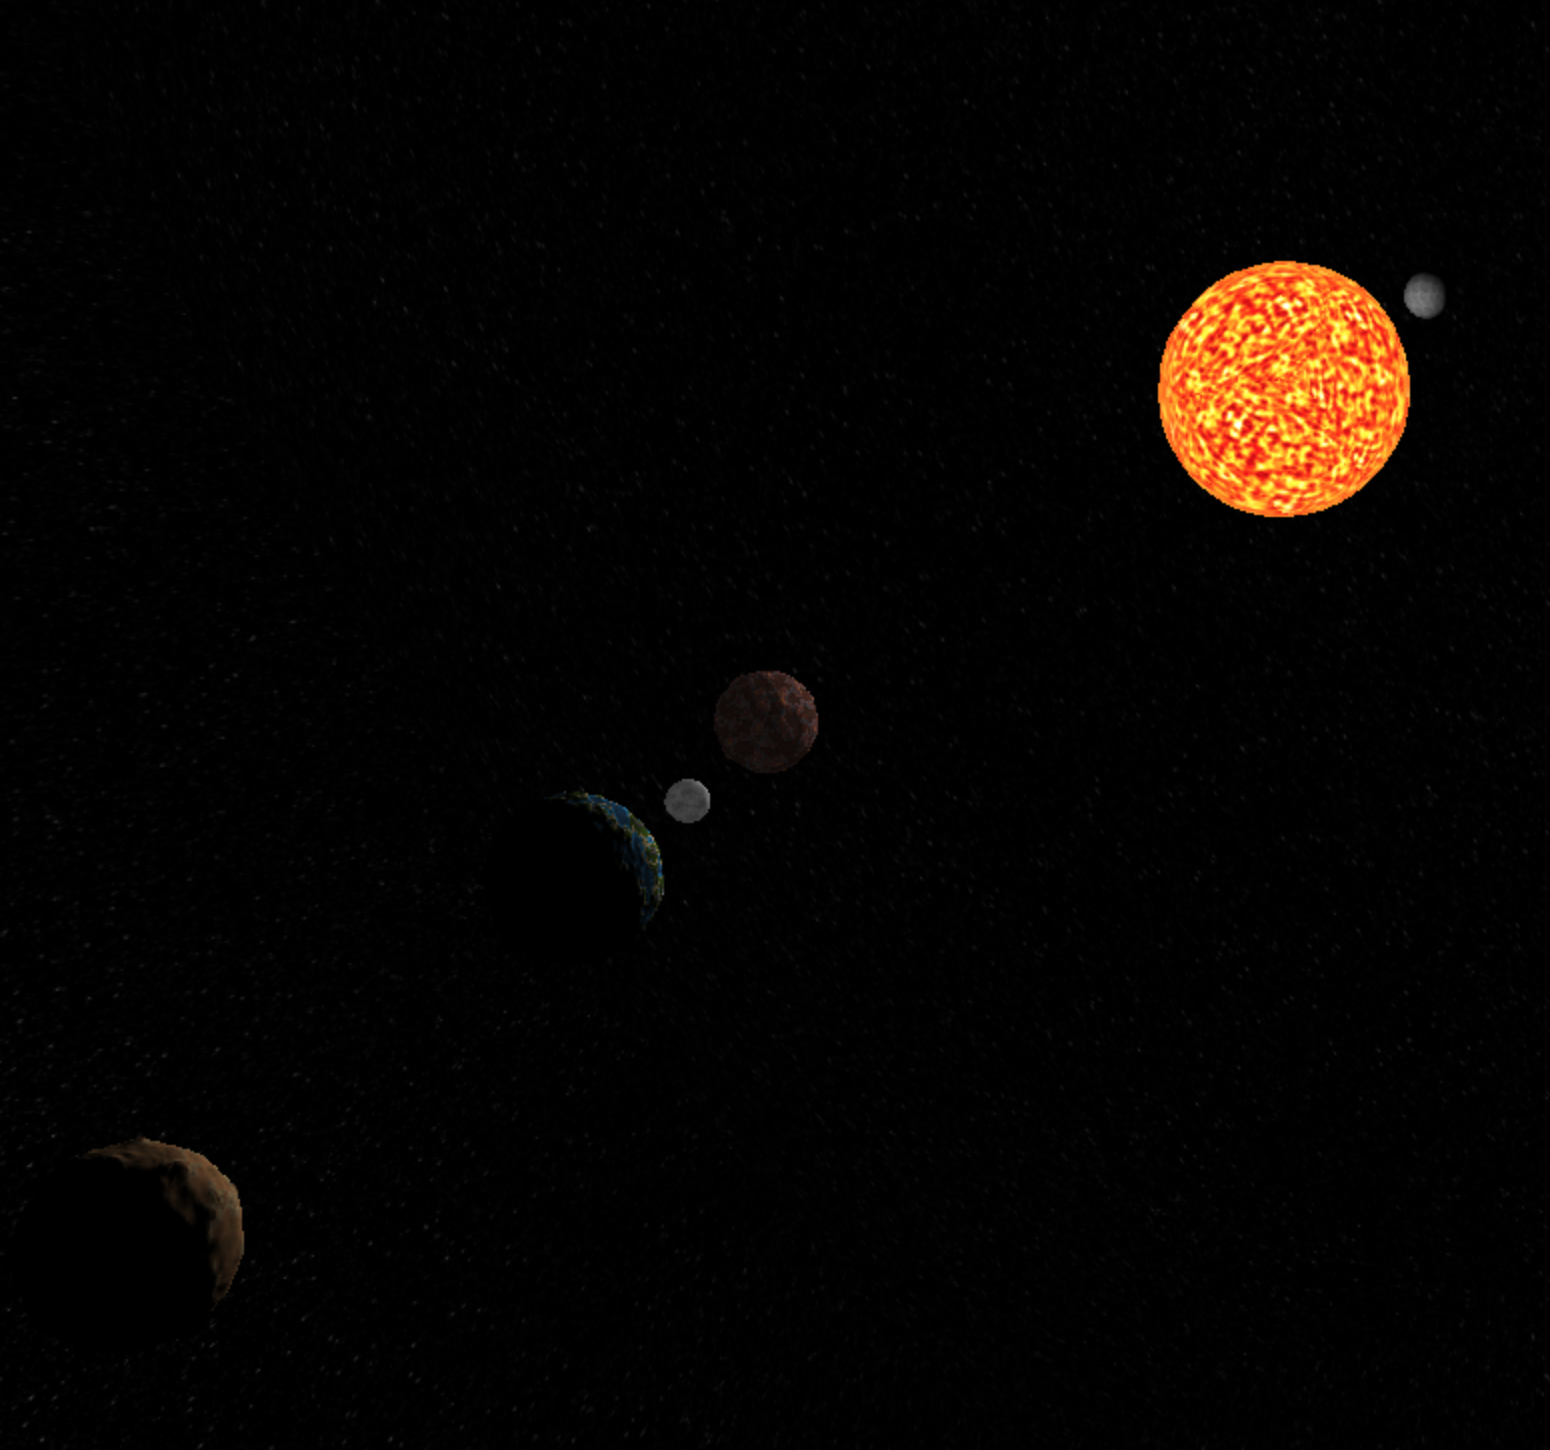
\includegraphics[scale=0.22]{images/solar_system.png}
	\caption{The planets are rotating around the Sun while the Moon is
		rotating around the Earth.}
	\label{fig:solar-system}
\end{figure}

%----------------------------------------------------------------------------------------

\section{Shaders and Textures}

As said before, the shaders are made by hand. This design choise is due to
the fact that it becomes easier to manage the textures of the terrain.

In fact, the texture changes on the height of the fragment, which was previously
determined using Perlin noise. This is necessary to assign, for the example
of the Earth, sea textures to low
heights, grass and mountain textures, or snow, to higher heights, creating
more realistic planets and differentiating seas by plains and mountains.

Moreover, a texture for the ``background'' is used, mapping a starfield on a
spherified cube, instead of a sphere, to solve, again, stratching of the image at the poles.

%----------------------------------------------------------------------------------------

\section{Collisions}

As said before FlyControl allows to move freely inside the scene.
Nevertheless, if not properly controlled, it is possible to move the camera
inside the planets as well.
In order to solve this problem, the position of the camera is always double
checked to avoid collisions. Thus, the camera cannot move inside the planets.

To perform this operation efficiently, planets are treated as spheres. If,
for each planet, the distance is greater than an approximation\footnote{The bounding sphere must have a radius greater than the radius of the corresponding planet plus an additional distance to cover the mountains.} of the corrispondent radius then there isn't any collision to handle, otherwise the camera position is reevaluated.\\
The new position of the camera is computed in two steps. First, the direction of the line that connects the camera to the planet is computed, then the camera is placed at a limit distance from the planet. This new position belongs to the line that pass through the planet centre and has the same direction as the one computed in the first step.\\
Note that the whole computation is independent from FlyControl and it can handle both the situation where the user go towards a planet and the inverse situation where a planet moves towards the camera. In the latter case, according to this position reevaluation, the camera would be moved away without enter inside 
the planet.\\
This technique is also used to prevent the user to go out of the space sphere\footnote{The space sphere represent starfield of the scene.}. Here the
position is recomputed coverserly to the previous case. Since the camera must be inside the box, the distance between its position and the world origin must be lower than the radius of the space sphere.

%----------------------------------------------------------------------------------------

\section{Planets Labels}

To improve the navigation inside the solar system, descriptive labels
were added to the scene. Each label shows the name and the type of the
object associated with it (e.g. Sun - Yellow Dwarf).
Basically these labels, placed near the associated object, are simple textured planes that keep looking in the direction of the camera. To achieve this result, a label is placed on the line that passes through the camera and the corresponding planet, at a fixed distance from the latter. The label is then rotated towards the camera
keeping the rotation on the z-axis fixed.

Since the labels are objects of the scene, they are subject to the projective
transformation made by the camera. Normally as the distance from the camera increase then the labels would look smaller. Labels are thus scaled with respect to their distance from the camera (i.e. closer labels have a smaller scaling factor than the further ones), making them look the same size.
Moreover, the opacity of the labels change according to the camera distance.
When the camera is moving towards a label, reached a certain threshold distance,
it starts to become more and more
transparent until it completely dissapears.
In this way a label never hides its planet when the camera is close to it.

Each label is drawn using a specific texture, which is not loaded from the
storage but it's created at runtime. This allows a better customization of the
information contained in each label.

The textures creation is executed using the HTML5 canvas components. Initially the planet informations and the tag background are drawn inside the canvas, then a Texture object is built from the canvas content. The new texture is finally passed as a uniform to the fragment shader in order to be rendered.\\
Figure \ref{fig:labels} shows a label associated to its planet.

\begin{figure}
	\centering
	\begin{subfigure}{.4\textwidth}
		\centering
		\includegraphics[width=1.0\linewidth]{images/labels_far.png}
	\end{subfigure}
	\begin{subfigure}{.4\textwidth}
		\centering
		\includegraphics[width=1.0\linewidth]{images/labels_near.png}
	\end{subfigure}
	\caption{Several views of the labels associated to the planets}
	\label{fig:labels}
\end{figure}

%----------------------------------------------------------------------------------------

\section{Earth's Ocean and Atmosphere}

The previously introduced procedural planet system deals with the generation of mountains and valleys for celestial bodies; at the top of that textures are applied in order to give to the planets or stars a more suitable appereance. However planets like Earth may have additional features such as an atmosphere or oceans; in the created solar system these features of the Earth were implemented using simple sphere meshes rendered with a Phong shader. For the oceans rendering it has been used a transparent blue sphere with a different shininess with respect to the ground. A texture mapped sphere was used for the atmosphere: the texture is a semi-transparent image of the Earth's clouds.\\
The ocean and atmosphere spheres were then added as child to the Earth object; to give a little animation to these entities, they didn't rotate as the parent do: in this way clouds will rotate around the planet and oceans will show some movement due to the imperfection of the sphere geometry.

%----------------------------------------------------------------------------------------

\section{Sun Particle Effects}

Until now the presented graphical objects do not show any particular effect, showing a static appeareance apart from the LOD system and the movement animation. For this reason a custom particles system was implemented with the aim of simulating a simple solar activity.\\
The basic idea is to add a high number of moving particles around the surface of the sun; more precisiously every particle move from the surface of the star to the outer space and disappear after having traveled for a fixed distance.\\
This effects makes sense if thousands of small particles are used; in order to achieve this result, keep the particles as simple as possible is absolutly essential: for this reason each particle of the system is composed by only one triangle.\\
However using thousands of objects, even if constructed with a single triangle, is still not possible: the 3D management of such a large number of elements, the enormous number of draw call needed and the increased communication between cpu and gpu will drastically compromise the performances of the webgl application.\\
The goal is then to minimize these compuations; a solution suitable to the described situation is to incorporate all the particles inside one geometry so to draw the particles system with only one draw call at render time.\\
It is important to remember that each particle moves independetly from the others so it is not possible to compute the right position from the cpu without modify the mesh geometry and loose in performance. For this reason all the particles are initialized in the same position (origin of the mesh) and then repositioned in their right position directly inside the vertex shader.\\
The set of informations required by the vertex shader for the particles placement includes movement direction, speed, scale, angular speed for each particle and the starting and ending movement distance from the centre of the entire system.\\
The information about each particle are concatenated and stored inside attribute buffers while the shared data like the distance range or the frame time are passed with uniforms. In THREE.js the only way to specify attribute buffers is by using a custom THREE.BufferGeometry which forces rewriting also the vertex, normal and UVs buffers. For the sun particles effects, normals and lights weren't use in the fragment shader considered the massive quantity of light emitted by a star: each particles is rendered from a semi-transparent texture\footnote{The texture has a semi-transaprent white drawing that is multiplicated with the random color of the particle.} colored with a random shade between yellow, orange and red.\\
In conclusion, using the tecnique just described it was possible to render up to a million indipendent particles (i.e. one million triagles) but in order to optimize the performances this number has been reduced to 100 thousands elements.

\begin{figure}
	\centering
	\begin{subfigure}{.4\textwidth}
		\centering
		\includegraphics[width=1.0\linewidth]{images/meteorites_near.png}
	\end{subfigure}
	\begin{subfigure}{.4\textwidth}
		\centering
		\includegraphics[width=1.0\linewidth]{images/meteorites_near.png}
	\end{subfigure}
	\caption{Sun with and without the particles effects}
	\label{fig:meteorites}
\end{figure}

%----------------------------------------------------------------------------------------

\section{Asteroids cloud}

After the four planet of the solar system, in the outer zone of the scene it was inserted a cloud of asteroids. The cloud is composed by several asteroids which move circularly around the sun, each with a different speed and at different distance from the center; to reach a more realistic visual effect, every asteroid has also a different rotation speed, scale factor and geometry. With regard to the last property, there were used about one hundred randomly deformed THREE.SphereGeometry: the deformation includes a random translation from the center of each vertex and a random scaling of the whole mesh on the three axis. During the creation of the cloud one of these deformed geometries is then assigned to each asteroid.\\
Due to the high number of object desired inside the cloud, the idea behind the implementation of the cloud is similar to the one of the sun particles system: in this case it is possible to consider an asteroid as a single particle while  the entire cloud is made up with a unique mesh.\\
Here a particle is clearly not built from a triangle alone but instead using a more complex mesh; in the BufferGeometry it was necessary to build the buffers related to vertices, normal and texture mapping by concatenating the equivalent buffers from the geometries associated with all the asteroids; furthermore, as in the case of the sun particles, additional buffers were created in order to provide to the shader extra informations for the asteroids' appearence and behaviour.\\
The informations regarding each asteroid are computed once at initialization time without any further computations excepts for the updates of the uniforms: for example at every animation frame the \textit{time} uniform is updated and then used in the vertex shader for calculating the right position and rotation of the asteroids in according with the informations stored in the attribute buffers.\\
Differently from the particles system used for the sun, here the rendering of each asteroid requires the use of lights and normals. Considering that all the asteroids are part of a single mesh, it hasn't been possible to use the modelView and normal matrices calculated by THREE.js. In this situation the modelView matrix is computed directly inside the vertex shader and the same is for the normal matrix; usually the normal matrix is computed as the transpose of the inverse of the modelView matrix but this technique would results in a higher load for the gpu so, considering that there isn't any non-isotropic scaling\footnote{Asteroids' geometry are subjected to a non-isotropic scaling during the sphere deformastion phase and normals are computed after this mesh transformation. Then, in the vertex shader, each asteroids is isotropically scaled. Isotropic scaling does not make the normals incorrect.} in the shader, it has calculated as the 3x3 upper left matrix of the modelView.\\
The advantages of the described approach is to draw in the scene up to several thousand meshes with a single webgl draw call, decreasing the number of communications with the GPU and lightening the cpu load.\\
A graphical representation of the introduced custom geometry can be seen in figure \ref{fig:buffer_geometry} while a sneak peak of the asteroids cloud is show in figure \ref{fig:meteorites}.

\begin{figure}
	\centering
	\begin{subfigure}{\textwidth}
		\centering
		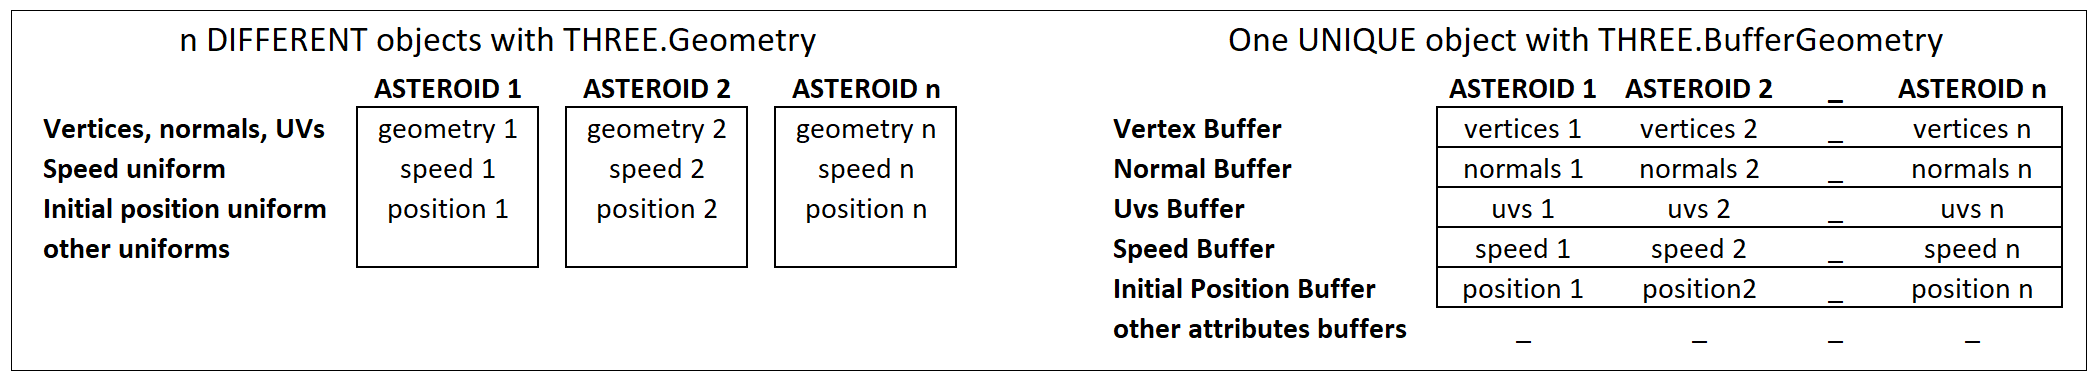
\includegraphics[width=1.0\linewidth]{images/asteroids_geometry.png}
	\end{subfigure}
	\caption{Comparison between \textit{n} single geometry and one BufferGeometry}
	\label{fig:buffer_geometry}
\end{figure}

\begin{figure}
	\centering
	\begin{subfigure}{.4\textwidth}
		\centering
		\includegraphics[width=1.0\linewidth]{images/meteorites_near.png}
	\end{subfigure}
	\begin{subfigure}{.4\textwidth}
		\centering
		\includegraphics[width=1.0\linewidth]{images/meteorites_near.png}
	\end{subfigure}
	\caption{Two views of the implemented cloud of asteroids}
	\label{fig:meteorites}
\end{figure}
%----------------------------------------------------------------------------------------

\section{Menu}

In addition to the use of the FlyControl, the user can interact with the program also through a simple gui menu. This is was implemented using a third party library called \textit{dat.GUI} \cite{datgui} which offers different input controls like buttons, checkbox, combobox, sliders and text inputs; moreover all of these can be grouped in folders. In order to implement a menu with dat.GUI is necessary to give at each desired control an initial value and extra informations about its behaviour: for example, a button needs a event listener, a slider needs a numerical range while a combobox needs a list of items. Note that the control type is not specified but indeed is automatically detected from the given extra information.\\
In this application the overlay provides input controls useful to manage the time speed or handle the camera position. In fact, through the apposites buttons it is possible to rotate or move the camera toward each planet of the solar system.
As shown in figure \ref{fig:menu}, every input control is placed in a folder based on his scope: folders in dat.GUI are basically openable and closable menu.\\

\begin{figure}
	\centering
	\begin{subfigure}{.4\textwidth}
		\centering
		\includegraphics[width=1.0\linewidth]{images/menu_open.png}
	\end{subfigure}
	\begin{subfigure}{.4\textwidth}
		\centering
		\includegraphics[width=1.0\linewidth]{images/menu_closed.png}
	\end{subfigure}
	\caption{Opened and closed dat.GUI menu}
	\label{fig:menu}
\end{figure}

%----------------------------------------------------------------------------------------

\section{How to Use}

Before launching the HTML file on the browser, it's necessary to execute a
server to load external files directly from the Javascript files. This can be
easily done with Python: \texttt{python3 -m http.server}.

The server will be created on port 8000, if available. It's then possible
to load the HTML file from \texttt{http://localhost:8000/main.html}.

The program has as inputs the inputs managed by the fly controller, which are:

\begin{itemize}
	\item \texttt{W}, \texttt{A}, \texttt{S}, \texttt{D}, mouse: move
	\item \texttt{R}, \texttt{F}: up/down
	\item \texttt{Q}, \texttt{E}: roll
	\item up, down: pitch
	\item left, right: yaw
\end{itemize}

With the mouse it is possible to use the overlay menu.

%----------------------------------------------------------------------------------------

\section{Third party elements}

%----------------------------------------------------------------------------------------

\section{Conclusion}

Procedural graphics in the last years have seen a big adoption in both videogames
and movie industry, this project is just an example of what can be done using
a simple tool like Perlin noise.

The creation of a complex planet full of details is not straightforward, even
by using tools made available by a library like THREE.js. Optimizing the structure of the program, in particular using chunks and
level of details is a must to deal with large terrains and with a high number
of meshes.

THREE.js simplifies the management of objects like planets and lights, making
it easy to manage the scene; moreover, having a large number of tools, like
different geometries and controls, speeds up the development of the project,
allowing the developers to concentrate more on the details of the program
than the structure of it.

%----------------------------------------------------------------------------------------

\newpage
\bibliography{bibliography}
\bibliographystyle{ieeetr}

%----------------------------------------------------------------------------------------

\end{document}
\grid
\grid
